\section{Fluxionnel execution model}

\subsection{Fluxions}

The fluxionnel execution model role is to manage and invoke autonomous execution units.
An execution units as we define it, accept only streams as input and output, that is a continuous and infinite sequence of data contained in messages.
We named this execution unit a fluxion.
That is a function, as in functional programming, only dependent from data streams.
It's composed of a unique name, a processing function, and a memory context during its execution.

Messages are composed of the name of the recipient fluxion, a body, and are carried by a messaging system.
After processing a message, the fluxion modify its context, and then terminate its execution by sending a message on its output stream.
Each fluxion send back a unique message to one or many recipient.
The fluxion's execution context is the set of state variables whose the fluxion depends on.

The fluxions make up a chain of processing binded by data streams.
All these chains make up a directed graph, managed by the messaging system.


% Le modèle d'exécution fluxionnel a pour fonction de manipuler et d'invoquer des unités d'exécutions autonomes n'ayant pour paramètre d'entrée et de sortie que des flux, c'est à dire des séquences continues et infinies de données agrégées par messages.
% Nous avons appelé ce type d'unité d'exécution autonome une fluxion.
% C'est à dire une fonction, au sens de la programmation fonctionnelle, dépendant exclusivement de flux de données.
% Elle est composée d'un nom unique, d'une fonction de traitement, et d'un contexte mémoire au moment de son exécution.

% Les messages sont composés du nom de la fluxion destinataire et d'un corps, et acheminés par un système de messagerie.
% % Ils représentent à la fois le signal d'invocation, et les données nécessaires à cette invocation.
% Après avoir traité un message, la fluxion modifie son contexte local, puis termine son exécution en renvoyant un message sur son flux de sortie.
% Chaque fluxion renvoie un message unique à destination d'une ou plusieurs fluxions.
% Le contexte d'exécution de la fluxion est composé de l'ensemble des variables d'état dont dépend la fluxion.

% Les fluxions forment des chaînes de traitement liées par les flux.
% L'ensemble de ces chaînes forme un graphe direct orienté, géré par un système de messagerie.

\subsection{Système de messagerie}

Le système de messagerie est le cœur du modèle d'exécution fluxionnel.
Il a pour fonction, à la fois d'acheminer les messages, et d'invoquer les fluxions.

Il est construit autour d'une file de messages, traités les uns après les autres par invocation de la fluxion destinataire.
L'utilisation d'une file de messages permet d'exécuter plusieurs chaînes de traitement parallèlement et équitablement, sans faire de différence dans l'ordonnancement entre messages locaux et messages provenant du réseau.
Le cycle de vie d'une application fluxionnelle est illustré figure \ref{fig:messagerie}.

\begin{figure}[h!]
  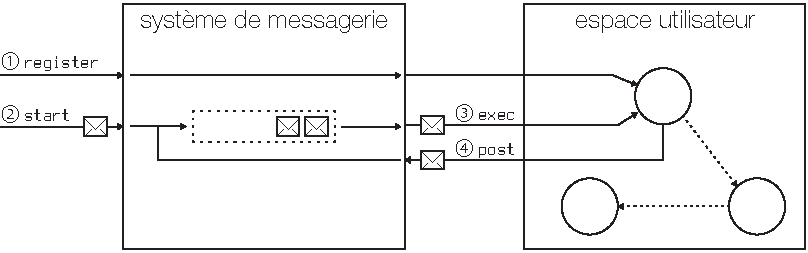
\includegraphics[width=\linewidth]{schema-message.pdf}
  \caption{Schema du système de messagerie}
  \label{fig:messagerie}
\end{figure}

Chaque fluxion dois être enregistrée dans le système de messagerie.
Cet enregistrement associe une fonction de traitement à un nom, et un contexte d'exécution initial.
Le système de messagerie achemine les flux de messages en se basant sur les noms des fluxions.
C'est pourquoi il ne peut pas exister deux fluxions ayant le même nom.
% Lors de cet enregistrement, il est possible d'initialiser le contexte d'exécution.
L'enregistrement se fait à l'aide de la fonction \texttt{register(<nom>, <fn>, <contexte>)}, étape \circled{1} sur la figure \ref{fig:messagerie}.
% Une fluxion peut elle-même enregistrer d'autres fluxions dynamiquement.

Pour déclencher une chaîne de fluxions un premier message est envoyé dans le système de messagerie, en utilisant la fonction \texttt{start(<msg>)}, étape \circled{2}.
Cette fonction va placer un premier message dans la file.
Le système dépile ce message, et exécute la fonction de traitement destinataire, étape \circled{3} et \circled{4}.
Le message résultat de cette exécution est alors empilé dans la file de message, étape \circled{5} et \circled{6}.
Le système boucle alors sur les étapes \circled{3} à \circled{6} jusqu'à ce qu'il n'y ai plus de messages dans la file.

Les algorithmes \ref{alg:traitement} et \ref{alg:parcours} formalisent précisément le comportement du système de messagerie généré suite à l'appel de la fonction \texttt{start}.

\begin{algorithm}
\caption{Algorithme de la file de messages}
\label{alg:traitement}
\begin{algorithmic}
\Function{processMsg}{$msg$}
\For{$dest$ \textbf{in} $msg.dest$}
\State $fluxion \gets lookup(dest)$
\State $message \gets$ \Call{exec}{$fluxion, msg.body$} \Comment{\circled{4} \& \circled{5}}
\State \Call{enqueue}{$message$} \Comment{\circled{6}}
\EndFor
\EndFunction
\end{algorithmic}
\end{algorithm}

\begin{algorithm}
\caption{Algorithme de parcours de la file}
\label{alg:parcours}
\begin{algorithmic}
\Function{loopMessage}{\null}
\While{$msg$ \textbf{presents in} $msgQueue$}
\State $msg \gets$ \Call{dequeue}{\null} \Comment{\circled{3}}
\State \Call{ProcessMsg}{$msg$}
\EndWhile
\EndFunction
\end{algorithmic}
\end{algorithm}

\subsection{Interfaces externes}

Afin de pouvoir interagir avec le monde extérieur, on définit des interfaces de bordures externes.
Notre approche repose sur les architectures Web.
L'interface externe permet de communiquer avec un client REST \footnote{REST: \textbf{Re}presentational \textbf{S}tate \textbf{T}ransfer \cite{Fielding2002}}.
Nous définissons dans cette interface deux composants :

\begin{itemize}
	\item[\textbf{In}]
    permet de recevoir des connections clientes.
    % C'est donc le premier maillon de la chaîne de traitement.
    Pour chaque connexion entrante, ce composant va transmettre l'identifiant de connexion au composant \textbf{Out}, lui permettant de répondre.
    Il transmet ensuite un message contenant l'identifiant de connexion et la requête à la première fluxion de la chaîne de traitement en appelant la fonction \texttt{start}.
	\item[\textbf{Out}]
    permet d'envoyer le résultat de la chaîne de traitement au client Web.
    Afin de recevoir les messages de la chaîne, le composant \textbf{Out} est enregistrée dans le système de messagerie sous le nom réservé \texttt{out}.
    % C'est donc le dernier maillon de la chaîne de traitement.
\end{itemize}


La figure \ref{fig:schemaweb} illustre les éléments spécifiques de cette interface Web au sein du système fluxionnel illustré par la figure \ref{fig:messagerie}.

\begin{figure}[h!]
	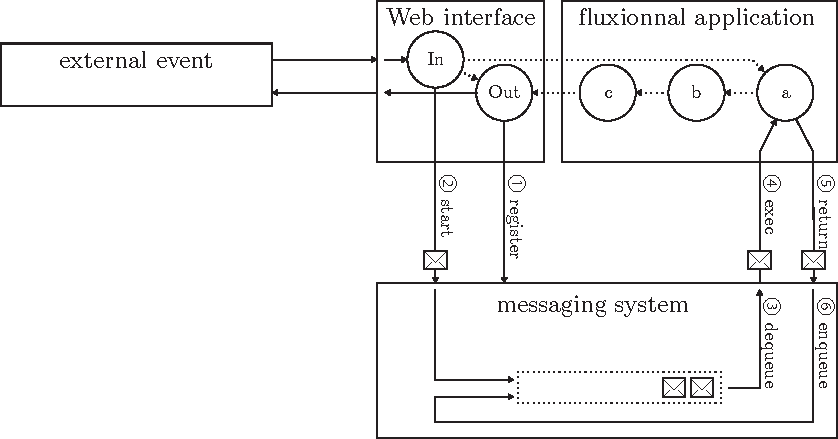
\includegraphics[width=\linewidth]{schema-web.pdf}
	\caption{Schema d'un système fluxionnel avec une interface Web}
	\label{fig:schemaweb}
\end{figure}

% TODO paragraphe de transition

\subsection{Exemple de service}

Afin d'illustrer le modèle d'exécution fluxionnel, nous présentons ici un exemple de son utilisation à travers un simple compteur de visites.
Ce service compte le nombre de connexions HTTP de chaque utilisateur et lui renvoie ce nombre dans la réponse.

La version initiale du service pourrait ressembler à l'extrait de listing \ref{lst:classique}.

\begin{code}[Javascript, caption={Service initial},label={lst:classique}]
var app = require('express')();

@\label{lst:classique_count}@var count = {};

@\label{lst:classique_get}\label{lst:classique_replyb}@app.get('/:id', function reply(req, res){
  count[req.params.id] = count[req.params.id]  || 1;
  ++count[req.params.id]
  var visits = count[req.params.id];
  var reply = req.params.id + '[' + visits + ']';
@\label{lst:classique_send}@  res.send(reply);
@\label{lst:classique_replye}@});

port = 8080;
app.listen(port);
console.log("Listening port: "+port);
\end{code}

Dans ce code il est intéressant de distinguer 3 éléments.
\begin{itemize}
  \item La variable \texttt{count} à la ligne \ref{lst:classique_count} est une mémoire persistante permettant de compter le nombre de visites pour chaque identifiant d'utilisateur distinct.
  Elle sera donc transformée dans le notion de contexte d'exécution du système fluxionnel.
  \item La fonction \texttt{reply}, ligne \ref{lst:classique_replyb} à \ref{lst:classique_replye} réalise le traitement fluxionnel type que l'on souahite réaliser.
  \item Enfin les deux méthodes \texttt{get} et \texttt{send}, respectivement ligne \ref{lst:classique_get} et \ref{lst:classique_send}, permettent d'interagir avec le serveur Web.
\end{itemize}

Ce programme minimal serait transformé dans notre système en la chaîne de fluxions illustrés figure \ref{fig:fluxions}.

\begin{figure}[h!]
  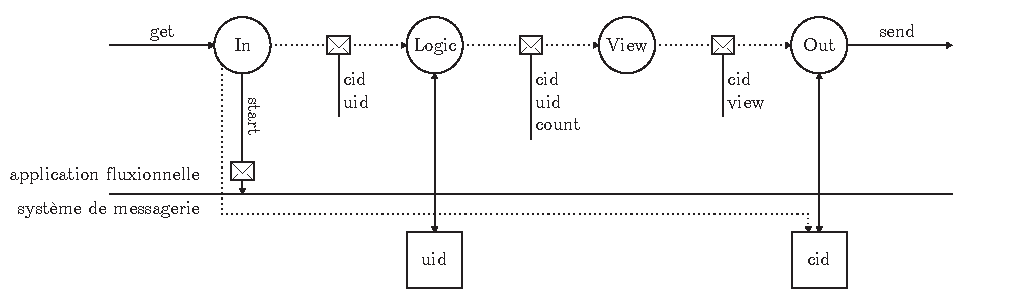
\includegraphics[width=\linewidth]{flux.pdf}
  \caption{Suite de fluxion du compteur}
  \label{fig:fluxions}
\end{figure}

L'extrait de code figure \ref{lst:fluxionnel} décrit ce même service de comptage dans un langage fluxionnel de haut niveau.
Ce pseudo code, de par la segmentation qu'il apporte par rapport au code initial, permet à un système annexe d'optimiser le placement des fluxions sur les machines physiques en fonction du coût des flux et de leur traitement.

Ce langage fluxionnel de haut niveau est non typé
\TODO{écrire un paragraphe sur les caractéristiques du langage, une subsection pourrait être nécessaire, mais elle serait peut être mieux placé dans la section sur la transformation}

\begin{code}[Javascript, caption={Code fluxionnel},label={lst:fluxionnel}]
use fluxion, web

fluxion input >> view
  this.uid[msg.uid] = this.uid[msg.uid] + 1 || 1
  msg.count = this.uid[msg.uid]
  return msg

fluxion view >> output
  msg.view = msg.uid + " connected " + msg.count + " times."
  msg.uid = undefined
  msg.count = undefined
  return msg

register input, {uid: {}}
register view

web.listen
\end{code}

Hormis les deux composants d'interface, le service à été segmenté comme suit :
\begin{itemize}
  \item La fluxion \texttt{input} est la première à recevoir le message du client.
  Elle contient l'ensemble de la logique de ce simple service.
  Pour des services réels, on trouverais à sa place l'ensemble des fluxions contenant la logique du service organisé en une ou plusieurs chaîne de traitement.
  Elle incrémente le compteur de l'utilisateur l'agrège au message, et renvoie ce dernier à la fluxion suivante.
  \item La fluxion \texttt{view} récupère le message, et met en forme la réponse que recevra l'utilisateur, et l'envoie à la fluxion de sortie.
\end{itemize}

% Ce service manipule principalement deux informations sur lesquelles qu'il est important de détailler.
% D'une part, les connections clientes sont partagé entre l'entrée et la sortie.
% Pour chaque connexion, l'entrée passe directement à la sortie un couple <id, res>.
% id représente simplement un identifiant permettant de retrouver res, il est envoyé à la fluxion input.
% res est la structure permettant de répondre au client.
% Ce mécanisme provoque un échange important de donnée entre le point d'entrée et le point de sortie, et implique de passer l'identifiant sur toute la chaîne de traitement, jusqu'à sa réception au point de sortie.

% Les messages échangés contiennent principalement deux informations importantes : les identifiants d'utilisateurs, permettant d'incrémenter un compteur pour chaque utilisateur, et les identifiants de connexion, permettant de lier une suite de messages avec la structure contenant la connexion HTTP.
% Le point d'entrée, et le point de sortie du système doivent rester sur la machine où la connexion a eu lieu pour avoir accès à l'interface réseau, tandis que les autre fluxions n'ont pas cette obligation, et peuvent être migré.


% Cet identifiant de connexion est nécessaire au point de sortie pour associer le résultat reçu avec la connexion vers laquelle le renvoyer à l'utilisateur.
% Nous passons cet identifiant pour ne pas alourdir les échanges de messages avec la structure contenant la connexion HTTP.

% Ainsi, la fluxion de sortie reçois des messages provenant de deux fluxions : le point d'entrée




